\chapter{Implémentation de la Kinect}

L'implémentation de la partie Kinect suivra une architecture de type client/serveur. Une partie serveur qui détecte les mains et qui envoie les positions via le réseau et une partie client, interne à WabinPaint, qui récupère la position des deux mains et les propage dans WabinPaint.

\section{Serveur}

La partie serveur est composée de deux parties, une parties acquisition des coordonnées des mains et une partie transmission sur le réseau.

\subsection{Récupération des coordonnées}
La société PrimeSense met à disposition des librairies \cite{kinect} qui permettent d'obtenir facilement un squelette d'utilisateur quand une personne est detectée. Grâce à ce squelette, nous pouvons accéder facilement aux données d'un bras, d'une jambe ou encore les mains. Notre serveur aura pour but de récupérer la position 3D (x,y,z) des mains de l'utilisateur. 

\subsection{Transmission des données, OSC}

Pour transmettre les données aux clients il a été choisi d'utiliser le réseau. Ce choix permettra de ré-utiliser la partie serveur pour d'autres applications.

La librairie Open Sound Control \cite{osc} a été choisie pour effectuer le transfert des données. Autrement appelé OSC, c'est un format de transmission de données entre ordinateurs, synthétiseurs, robots ou tout autre matériel ou logiciel compatible, conçu pour le contrôle en temps réel. OSC utilise le réseau au travers des protocoles UDP ou TCP.  

\newpage

OSC permet avec simplicité d'envoyer des données, comme visible ci-dessous:

\begin{lstlisting}
	//Send positions
	lo_send(oscClient,"/pointers","ffffff", hand0_X, hand0_Y, hand0_Z, hand1_X, hand1_Y, hand1_Z);
\end{lstlisting}

Voici un aperçu des commandes nécessaire pour récupérer les données dans la partie client: 

\begin{lstlisting}
//Receive positions
	if (ktrack->oscProxy->receive() < 0) return false;
	bool newpos = ktrack->oscProxy->pointers_position(x0, y0, z0, x1, y1, z1);
\end{lstlisting}
	
\section{Client}

Concernant le client, comme il a été dit précédemment, WabinPaint implémente plusieurs types de tracker, avec en super classe un tracker générique permettant d'avoir accès à des méthodes propageant et traitant les données relatives au positionnement des mains. GenericTracker est une classe définissant un comportement minimal pour les classes de tracking. KTrack qui est la classe de tracking pour la Kinect hérite de GenericTracker. KTrack  permet donc de récupérer les données reçues sur le réseau et de les propager dans WabinPaint. 


\begin{figure}[!ht]
	\center
	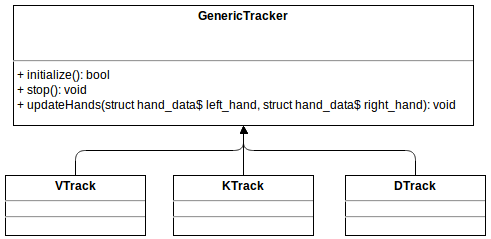
\includegraphics[scale=0.5]{image/ktrack_implement.png}
	\caption{Relations d'héritage entre périphériques de tracking}
\end{figure}

KTrack récupère les données du réseau grâce à la partie client OSC.

\section{Premiers résultats}

Par défaut, le mode de dessin est actif lorsque les deux mains sont jointes, mais cela provoque dans certains angles des erreurs de positions. En effet, lorsqu'une main masque l'autre main, Kinect considère que la main masquée n'existe plus, ce qui renvoie des coordonnées erronées. Pour corriger ce problème, il a été proposé de changer le mode d'activation du dessin.

En plus du problème concernant le déclenchement du mode de dessin, il a été observer que les données recu de la Kinect sont bruitées. Ce bruit a pour résultat un tremblement du curseur et donc une imprécision lors des dessins.

Voici une illustration de l'effet du bruit sur le dessin :


\begin{figure}[!ht]
	\center
	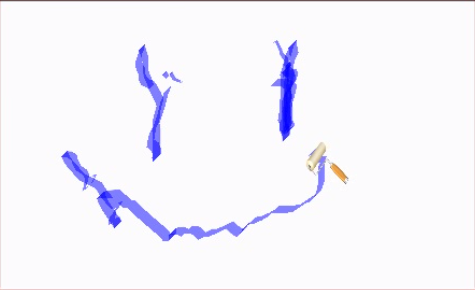
\includegraphics[scale=0.5]{image/bruit.png}
	\caption{Dessin d'un smiley, bruitage trop important}
\end{figure}

Dessiner une figure est très compliqué avec le bruit comme visible sur le dessin du smiley.
 

